\chapter{Testing with a transition system}\label{sec:topic_3}

\section{Introduction}

System tests are used to make sure that clients receive exactly the kind of software they previously specified within the order contract submitted to the software vendor. Oftentimes what was specified and what was implemented does not match entirely in the end. The software vendor faces traceability problems to track which requirements could be covered in which tests and therefore which requirements got implemented. How does one make sure that each atomic functional and robustness requirement specified is covered in the requirements' implementation?

To solve this, the process of formal definition of requirements and matching system tests must be brought closer together. Testing should already be possible in early stages of development, to be precise during the specification phase already. To automatically derive test scenarios from means of the specification area \textit{transition systems} are used. They help to generate test paths as possible combinations of fine-grained functional requirements received through the traversal. An equivalent approach can be used to derive robustness tests as well. In this process requirements can furthermore be tested on their consistency, correctness and integration and eventually can be refined further.

For this purpose the two approaches \cite{ClementineNebut2006} and \cite{NajlaRaza2007} were analyzed. While \cite{ClementineNebut2006} was given in advance by the advisors, \cite{NajlaRaza2007} was discovered through an extensive literature search shown in \autoref{literaturesearch}. Both approaches will be explained in the following sections \autoref{approachone} and \autoref{approachtwo} and applied to the movie management software example. A comparison between the two approaches will be drawn using a synthesis matrix shown in \autoref{comparison}. The main results of testing with transitions systems will be summarized in \autoref{conclusion}. 

Please refer to the glossary in order to receive a common understanding of the following terms used in the sections below: contract, coverage criterion, interaction overview diagram, object constraint language, operation, test case, test objective, test scenario, transition system, UC-System, UC-SCSystem, use case, use case scenario, XML metadata interchange.

\section{Literature search} \label{literaturesearch}

The literature research was driven by the central research question (RQ): 

\glqq Which approaches for automatic generation of system tests exist that are using contract enriched use cases or other use case related means of the specification area within a transition system simulation model?\grqq 

The focus during this literature search was on finding a second approach to automatically generate system tests from means of the specification phase by exhaustively simulating a transition system to generate test paths similar to \cite{ClementineNebut2006}. But as \cite{ClementineNebut2006} is restricted on using \textit{contract} enriched \textit{use cases} and \textit{use case scenarios}, the way how \textit{test objectives} are derived was this time freely selectable to receive another new, but similar approach. The pre-search results were promising both on IEEE Xplore and ACM. Only some papers on ACM could not be accessed publicly. The number of results was considered to be sufficient to cover all relevant scientific papers, which is why the research was restricted on these two platforms. Furthermore, two relevance criteria inspired by the central RQ were defined:

\begin{itemize}
	\item Does the method described in the article generate system tests automatically from use cases or other use case related means of the specification area?
	\item Are test objectives generated using some kind of simulation model based on use case contracts (pre- and postconditions) or similar transition system approaches?
\end{itemize} 

As system tests can not exclusively be derived from means of the specification area, an article should restrict to generating system tests from use case related means of the specification area. To derive test objectives a transition system should be simulated exhaustively based on contract definitions (pre- and postconditions). 

The search was done using both snowballing and search term techniques. 140 papers were found referencing \cite{ClementineNebut2006} and 46 articles were referenced by \cite{ClementineNebut2006}. The results of the snowballing search can be found in \autoref{snowballing}. The backward snowballing approach was restricted on references stated in the \textit{Related Work} chapter as all other references relate to preceding work that serve as basic knowledge to realize the transition system approach in \cite{ClementineNebut2006}. Additionally, most of the references were quite old since the original paper was published in 2006. Therefore not all papers could be found on IEEE Xplore or ACM, which is why the number of considered papers is even lower than the number of original references found. Why specific papers were considered not suitable or only partly suitable is documented in \cite{FelixHausberger2020}.

\begin{small}
	\begin{longtable}{l|c|c|c}
		\caption{Results of snowballing techniques}
		\label{snowballing}	
		\\    %%%%<===
		\hline
		 & \textbf{Yes} & \textbf{Possibly} & \textbf{No} \\
		\hline	
		Forward snowballing & 5 & 9 & 63 \\
		\hline
		Backward snowballing & 2 & 1 & 2 \\
		\hline
	\end{longtable}
\end{small}


Seach-term based search was done using the following key terms: system tests, automatic generation, transition system, simulation model, use cases, contracts. Only papers published between 2006 and 2020 having the search term \enquote{test} and \enquote{use case} in their publication title were evaluated. 

\newpage


\begin{longtable}[h]{c|c|p{0.2\textwidth}|p{0.2\textwidth}|c}
		\caption{Results of search-term based technique}
		\label{search-term}\setlength{\tabcolsep}{1em}\\
		\hline
		\textbf{Source} & \textbf{Date} & \textbf{Search restrictions} & \textbf{Search query} & \textbf{\#Results} \\
		\hline
		IEEE Xplore & 2020-11-21 & \enquote{system tests} in document title; \enquote{automatic generation} in document title; \enquote{transition system} in full text \& metadata; \enquote{simulation model} in full text \& metadata; \enquote{use cases} in document title; \enquote{contracts} in full text \& metadata; & \enquote{system tests} AND \enquote{automatic generation} AND \enquote{transition system} AND \enquote{simulation model} AND \enquote{use cases} AND contracts & 0 \\
		\hline
		IEEE Xplore & 2020-11-21 & \enquote{system tests} in document title; \enquote{automatic generation} in abstract; \enquote{transition system} in full text \& metadata; \enquote{use cases} in document title; \enquote{contracts} in full text \& metadata; & \enquote{system tests} AND \enquote{automatic generation} AND \enquote{transition system} AND \enquote{use cases} AND contracts & 0 \\
		\hline
		IEEE Xplore & 2020-11-21 & \enquote{test} in document title; \enquote{transition system} in full text \& metadata; \enquote{use cases} in document title & \enquote{system tests} AND \enquote{transition system} AND \enquote{use cases} & 82 \\
		\hline
		ACM & 2020-11-21 & \enquote{system tests} in title; \enquote{automatic generation} in title; \enquote{transition system} in full text; \enquote{simulation model} in full text; \enquote{use cases} in title; \enquote{contracts} in full text; & \enquote{system tests} AND \enquote{automatic generation} AND \enquote{transition system} AND \enquote{simulation model} AND \enquote{use cases} AND contracts & 0 \\
		\hline
		ACM & 2020-11-21 & \enquote{system tests} in title; \enquote{automatic generation} in abstract; \enquote{transition system} in full text; \enquote{use cases} in title; \enquote{contracts} in full text; & \enquote{system tests} AND \enquote{automatic generation} AND \enquote{transition system} AND \enquote{use case} AND contracts & 0 \\
		\hline
		ACM & 2020-11-21 & \enquote{system tests} in title; \enquote{transition system} in full text; \enquote{use cases} in title & \enquote{system tests} AND \enquote{transition system} AND \enquote{use cases} & 0 \\
		\hline
		ACM & 2020-11-21 & \enquote{test} in title; \enquote{use case} in title & \enquote{system tests} AND \enquote{use case} & 8 \\
		\hline
\end{longtable}

From the resulting papers, only one was considered suitable as a potential second paper. After the search for potential articles to be evaluated was finished, a choice between eight remaining papers from the initial search had to be made:

\begin{itemize}
	\item System Testing using UML Models \cite{MonalisaSarma2007},
	\item An Automatic Tool for Generating Test Cases from the System's Requirements \cite{RosziatiIbrahim2007},
	\item Automated Test Case Generation from Use Case: A Model Based Approach \cite{LizheChen2010},
	\item Requirements Document Based Test Scenario Generation for Web Application Scenario Testing \cite{XiaojingZhang2015},
	\item An Approach to Modeling and Testing Web Applications Based on Use Cases \cite{LipingLi2008},
	\item Test cases generation from UML state diagrams \cite{YGKim1999},
	\item Requirements by Contracts allow Automated System Testing \cite{ClementineNebut2003},
	\item An Automated Approach to System Testing Based on Scenarios and Operations Contracts \cite{NajlaRaza2007}.
\end{itemize}

The decision criteria are based on the different search terms mentioned above and the already defined criteria. Additionally, focus of the selected paper should lie on creating system tests for any generic application area, not just UI related parts of an application.

The paper \textit{An Automatic Tool for Generating Test Cases from the System's Requirements} was not chosen as it does not focus on testing the consistency of use case combinations with contracts to build test objectives as in the original paper. Furthermore, it is not as in-depth as the original paper. Contract enriched use cases could neither be found in \textit{System Testing using UML Models}.

\textit{Automated Test Case Generation from Use Case: A Model Based Approach} really embodies the principle of state base modeling based on use cases with its \textit{interaction finite automaton} (IFA), but doesn't introduce a formal language to define use cases and its contracts.

\textit{Requirements Document Based Test Scenario Generation for Web Application Scenario Testing} as well as \textit{An Approach to Modeling and Testing Web Applications Based on Use Cases} are specifically optimized for web application \textit{test scenarios} and therefore not as general and universally applicable as the original paper.

\textit{Test cases generation from UML state diagrams} and \textit{Requirements by Contracts allow Automated System Testing} could unfortunately not be accessed in full length in IEEE Xplore.

The chosen article to further evaluate is \textit{An Automated Approach to System Testing based on Scenarios and Operations Contracts}, as it introduces a second way to create system tests from use case scenarios as UML 2.0 models by enriching it with contracts and by transforming the formalized scenarios to a transition system to derive test objectives. It uses a more graphical approach to define use cases instead of using a formalized language to do so and goes deeper down into use-case level instead of system-level test generation. A more in-depth comparison between the two papers can be found in \autoref{comparison}.

\section{Approach 1: Automatic test generation: A Use Case driven approach} \label{approachone}

\subsection{Description}

\begin{figure}[h]
	\centering
	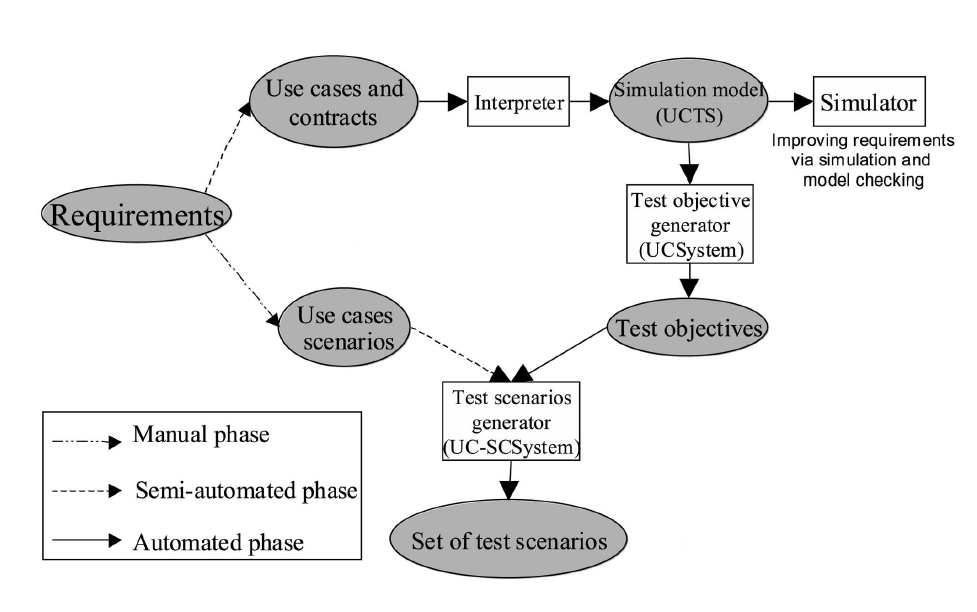
\includegraphics[width=0.75\textwidth]{../images/topic3_transitionsystemflow.png}
	\caption{Flow of generating test scenarios \cite{ClementineNebut2006}}
	\label{tsf}
\end{figure}

The approach consists of two phases (see \autoref{tsf}). In the first phase, UML use cases get enhanced with contracts (pre- and postconditions). Use cases can be seen as the systems' main functions whereas contracts are used to infer the correct partial ordering of functionalities that the system should offer. They express the ordering constraints between the use cases during the simulation process to build the transition system. The contracts are made executable for logical evaluation by writing them in the form of requirement-level first-order logical expressions. They consist of predicates with and are used to describe facts in the system like actor state, main concept state, roles, and more. Each predicate can either evaluate to true or false, but never to undefined. A dedicated editor tool helps to manage the predicates and guides the design of contracts to maintain a nonredundant, minimal set of contracts and predicates. Contracts therefore specify the system properties to make a use case applicable (preconditions) and define the system properties (predicates) acquired after their application (deterministic postconditions). Parameters to use cases can either be system actors or main concepts of the use case, which are represented as normal instantiated objects of classes during the test scenario generation process. 

Through exhaustive simulation by the prototype/interpreter-tool \textit{UC-System} a \textit{use case transition system} (UCTS) is built, which serves as a model for all valid sequences of use cases. Therefore first an initial state and enumerations of different business entities that later serve as parameters to use cases are declared. Then all use cases get instantiated by replacing the set of formal parameters with all the possible combinations of their possible actual values (i.e. actors and main concepts). To apply an instantiated use case the simulation state and the precondition of an instantiated use case must match. The simulation state is then updated according to the postcondition of the contract. The initial state defines which predicates are true from the very beginning, the current simulation state covers all instantiated predicates which are evaluated to true. Now all possible paths are traversed exhaustively until a final UCTS was generated. 

During this step, the requirement engineer has also the chance to check and possibly correct the requirements before the tests are generated. Inconsistencies between predicates and contracts can be identified as well as underspecification or errors in the requirements. Invariants can also be checked. The number of states in the transition system can be calculated with

\begin{equation}
	maxsize_{UCTS} = 2^{n_{ip}}
\end{equation}

where

\begin{equation}
	n_{ip} = p \cdot max_{instances}^{max_{param}}.
\end{equation}

$n_{ip}$ describes the amount of instantiated predicates, $p$ the number of predicates, $max_{instances}$ the maximum amount of instances for a parameter (actors and main concepts of the use case), and $max_{param}$ the maximum amount of parameters per predicate p. In practice, many of the potential states are not reachable and only a small number of instances are necessary for achieving a proper statement coverage. 

Now relevant test objectives get extracted from the UCTS by applying predefined \textit{coverage criteria}. 

The \textit{All Edges} (AE) criterion makes sure that all state transitions are covered, whereas the \textit{All Vertices} (AV) criterion guarantees that all states (predicates) are reached within the set of test objectives.  The \textit{All Instantiated Use Cases} (AIUC) criterion is helpful in case a state transition can be done by multiple use cases or a use case leads to no state change. A combination od AV and AIUC is the \textit{All vertices and All Instantiated Use Cases} (AV-AIUC) criterion. The most strict criterion is probably the \textit{All Precondition Terms} (APT) criterion, which makes sure that all possible ways to apply each use case are exercised. Now, these criteria are mainly introduced to generate functional tests. The \textit{Robustness} criterion on the other hand explicitly exercises a use case in as many different ways as to make its precondition false. Therefore valid test paths are generated, which lead to an invalid application of a use case to generate robustness tests from. All algorithms are based on breadth-first search in the UCTS to obtain small test-objectives that are human-understandable and meaningful. 

\newpage 

Subsequently, in the second phase, test scenarios get generated by replacing each use case in a test objective with the according use case scenario that is compatible in terms of static contract matching. This is done by the prototype-tool \textit{UC-SCSystem}. The use case scenarios were also attached with contracts beforehand. This time the contracts contain more detailed pre- and postconditions. There are contracts that rely on the rest of the model, they are written in \textit{Object Constraint Language} (OCL), and there are contracts that rely on the predicates of the use cases. Now the exchange of messages involved between the environment and the system is also specified. Note that all use case scenarios are system-level scenarios. Eventually, additional parameters and messages need to be passed manually before executable \textit{test cases} can be generated. The process results in executable test scenarios that get evaluated using the statement coverage metric.

One possible challenge of the approach is that the simulation model has to be compact enough to avoid combinatorial explosion of the internal states. Therefore the two-phase approach was chosen and parameters to instantiate use cases during the simulation can often be restricted to only the main system concepts and actors. Furthermore, the above-mentioned test objective generation criteria were identified through experimental comparisons and help to keep the number of test objectives in a reasonable scope. 

The generated test scenarios can either lead to a pass verdict, a fail verdict (in case a postcondition is violated), or an inconclusive verdict. The latter is invoked if a precondition is evaluated to false and the test scenario was not executed entirely. This could be because of underspecification or because of inappropriate test data. To solve this either a new initial state (test data) has to be defined or additional test cases that execute the remaining use case scenarios need to be provided. 

To evaluate the approach the original authors used three software products: An Automated Teller Machine (ATM) with 850 lines of code, an FTP server with 500 lines of code, and a virtual meeting (VM) server with 2.500 lines of code. Statistics on the amount of generated test cases can be found in \autoref{testcases}.

\begin{table}[h] 
	\centering
	\begin{small}
		\caption{Statictics of the generated test cases}
		\label{testcases}
		\setlength{\tabcolsep}{1em}
		\begin{tabular}{l|c|c|c}
			\hline
			& \textbf{ATM} & \textbf{FTP} & \textbf{VM} \\
			\hline
			\# use cases & 5 & 14 & 14 \\
			\hline
			\# nominal UC-scenarios & 5 & 14 & 14 \\
			\hline
			\# exceptional UC-scenarios & 17 & 14 & 14 \\
			\hline
			\# generated functional test cases & 6 & 14 & 15 \\
			\hline
			\# generated robustness test cases & 17 & 33 & 65 \\
			\hline
		\end{tabular}
	\end{small}
\end{table}

Taken the example of the VM server, most coverage criteria reached up to 70\% code coverage, when including robustness test cases even up to 80\%. For more detailed information see \autoref{codecoverage}.

\begin{table}[h]
	\centering
	\begin{small} 
	\caption{Statement coverage reached by the generated test cases}
	\label{codecoverage}
	\setlength{\tabcolsep}{1em}
		\begin{tabular}{l|c|c|c}
			\hline
			& \textbf{ATM} & \textbf{FTP} & \textbf{VM} \\
			\hline	
			\% of functional code covered & 100\% & 90.7\% & 100\% \\
			\hline
			\% of robustness wrt. the spec covered & 42.31\% & 38.6\% & 52\% \\
			\hline
			\% of code covered (total) & 94.76\% & 72.5\% & 80\% \\
			\hline
		\end{tabular}
	\end{small}
\end{table}

All coverage criteria are almost equal in their achieved code coverage, with the exception of the AV criterion. Here the code coverage is low as not all use cases can be covered, especially those use cases that do not change the system state are missing. The ratio between the covered statements and the amount of generated test cases gives information about the efficiency of the generated test scenarios. Here the AIUC and APT criteria scored best. The APT criterion manages to reach 100\% functional code coverage with only 15 test cases. The efficiency of the robustness criterion on the other hand scored quite low, 65 test cases could only cover up to 50\% of the equivalent robustness code. Therefore the approach works well for functional code, but not so well for robustness code. This is because only violations of the use case attached preconditions are taken into account, inappropriate test data, or violating the more detailed preconditions of use case scenarios are not included in the test generation process. 

One possible extension of the approach was also considered. Activity diagrams could be chosen to model the use case dependencies in a more graphical approach, which is then shown in the upcoming approach two. 

\subsection{Application}

In the first step, the test objectives have to be derived. Therefore we define the use cases and their contracts (\autoref{contracts1}) as requirement-level first-order logical expressions. The contracts are used to infer the correct partial ordering of functionalities that the system should offer. Only the use cases that really impact the state of the transition system were specified for this example. The notation used is equal to the one proposed in the paper. \textit{UC} introduces the identifier and parameters of a use case, \textit{pre} marks the beginning of the precondition logical expression and \textit{post} the beginning of the postcondition logical expression. Furthermore, logical operators like \textit{and} and \textit{or}, quantifiers like \textit{forall} and \textit{exists}, and implications by using \textit{implies} can be used. The expression \textit{@pre} ensures that a given logical expression has already been evaluated to true when evaluating the precondition. 

\begin{lstlisting}[caption={Contracts attached to use cases},label={contracts1}]
	
	UC createMovie(m: movie)
	post createdMovie(m)
	
	UC createLinkedPerformer(p: performer, m: movie)
	pre createdMovie(m)
	post createdPerformer(p) and createdLink(p,m)
	
	UC rateMovie(m: movie)
	pre createdMovie(m)
	post calculatedOverallRating(m)
	
	UC ratePerformer(p: performer)
	pre createdPerformer(p)
	post forall(m: movie){ createdLink(p,m)@pre implies calculatedOverallRating(m) }
	
	UC linkExistingMovie(m: movie, p: performer)
	pre createdMovie(m) and createdPerformer(p)
	post not createdLink(p,m)@pre implies (createdLink(p,m) and calculatedOverallRating(m))
	
	UC linkExistingPerformer(m: movie, p: performer)
	pre createdMovie(m) and createdPerformer(p)
	post not createdLink(p,m)@pre implies (createdLink(p,m) and calculatedOverallRating(m))
	
	UC unlinkMovie(m: movie, p: performer)
	pre createdMovie(m) and createdPerformer(p) and createdLink(p,m)
	post calculatedOverallRating(m) and not createdLink(p,m) and not exists(m2: movie){ createdLink(p,m2) }@pre implies not createdPerformer(p)
	
	UC unlinkPerformer(m: movie, p: performer)
	pre createdMovie(m) and createdPerformer(p) and createdLink(p,m)
	post calculatedOverallRating(m) and not createdLink(p,m) and not exists(m2: movie){ createdLink(p,m2) }@pre implies not createdPerformer(p)
	
	UC removeMovie(m: movie)
	pre createdMovie(m)
	post not createdMovie(m) and forall(p: performer){ not createdLink(p,m) } and not exist(m2: movie){ createdLink(p,m2) }@pre implies not createdPerformer(p)
	
	UC removePerformer(p: performer)
	pre createdPerformer(p)
	post not createdPerformer(p) and forall(m: movie){ not createdLink(p,m) and calculatedOverallRating(m) }
\end{lstlisting}

After that, the UC-System prototype/interpreter tool should build the UCTS (\autoref{ucts}) through exhaustive simulation. The pool of parameters was restricted to one movie and performer to avoid a combinatorial explosion for this example. To build instantiated use cases the set of formal parameters are replaced with all the possible combinations of their actual values. In our case, we use the most simple approach by just having one possible combination. Furthermore, the predicate calculatedOverallRating is no longer considered. Note that only predicates that evaluate to true are listed in the states as in the original paper. 

\begin{figure}[h]
	\centering
	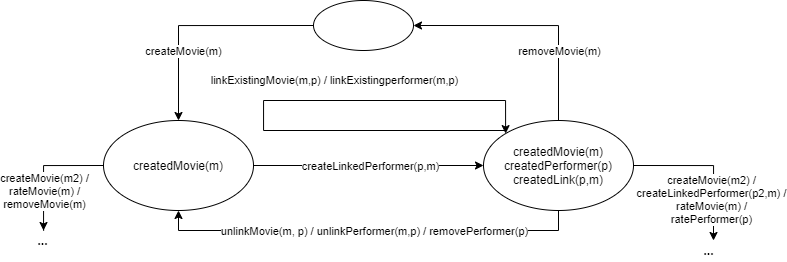
\includegraphics[width=0.85\textwidth]{../images/topic3_ucts.png}
	\caption{The use case transition system}
	\label{ucts}
\end{figure}

After applying an instantiated use case in the transition system (in case the precondition of the contract was fulfilled) the simulation state is updated according to the contracts' postcondition. 

\newpage

Depending on the selected coverage criterion, we receive different test objectives as correct sequences of use cases. The robustness criterion was not considered in this example, but its application is coherent to the functional coverage criteria. How many test objectives are derived depends on the internal implementation of UC-System and cannot be predicted for this example. Let's assume that one test objective is the test path createMovie(m) \mbox{-\textgreater} createLinkedPerformer(p,m) \mbox{-\textgreater} removeMovie(m). Then the use case scenarios from \autoref{ucs} are used to replace the use cases in the test objectives. It helps to specify the exchange of messages involved between the environment and the system.

\begin{figure}[h]
	\centering
	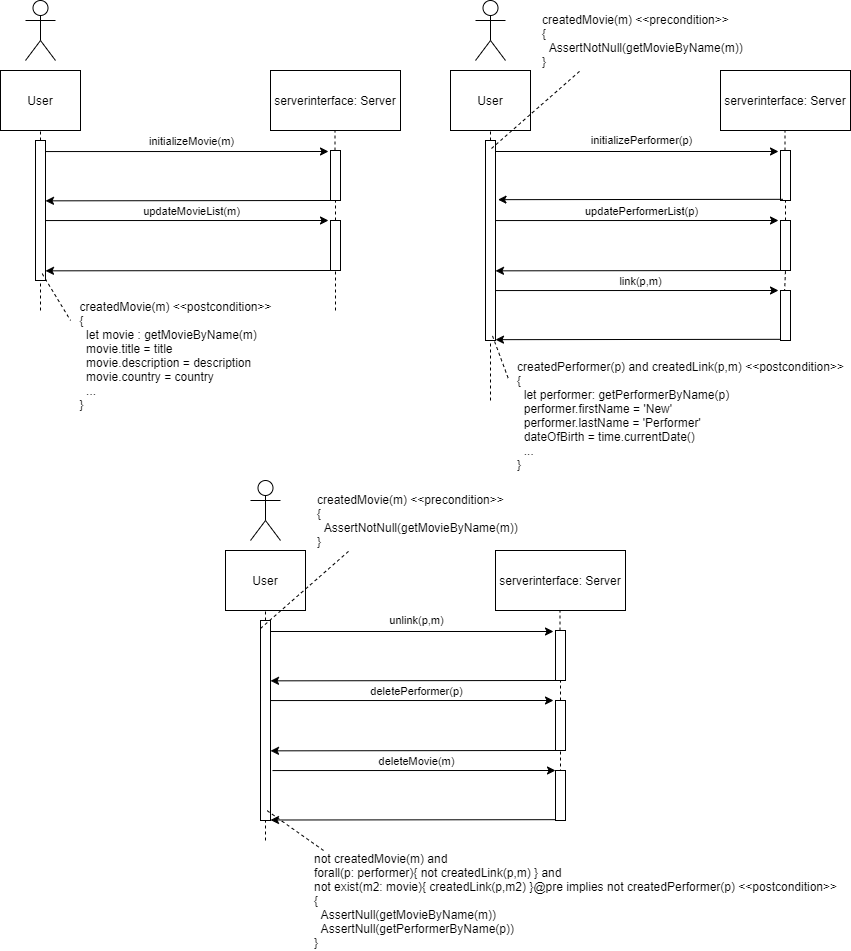
\includegraphics[width=1.0\textwidth]{../images/topic3_ucs.png}
	\caption{The use case scenarios}
	\label{ucs}
\end{figure}

\newpage
Note that the use case scenarios may still be incomplete for the execution. They contain the main messages exchanged between the tester and the SUT and say how the system has to be simulated to perform a use case and how to react to the simulation. To know how the system has to be simulated, the use case scenarios contain more detailed contracts written in OCL besides the contracts written as logical expressions that were provided by the use cases. 

The prototype-tool UC-SCSystem uses the shown implementation in the use case scenarios to derive executable test scenarios as JUnit tests.

\section{Approach 2: An Automated Approach to System Testing based on Scenarios and Operations Contracts} \label{approachtwo}

\subsection{Description}

Based on the suggested improvements in the first paper, the second paper uses a more graphical approach using \textit{interaction overview diagrams} (IOD), a special form of activity diagram used to show control flow, to derive test paths. It helps to start testing in the early stages of development. Each node in the IOD represents either an interaction diagram (sequence diagrams) or interaction occurrences that show an \textit{operation} invocation. Every IOD corresponds to one use case. The IODs get enhanced with contracts written in the \textit{object constraint language} (OCL) and they get transformed into a contracts transition system (CTS) which models all scenarios of the IOD. Here the states are represented by the contracts and the transitions by the operations (interaction diagrams or interaction occurrences) in the IOD. The CTS is built by a tool using the \textit{XML metadata interchange} (XMI) file for the IOD and the operation contracts in OCL as inputs. A state is created against each precondition and each postcondition of the operations. Logical if-then-else conditions are resolved by combining their testing condition with the result, therefore two different sub-states are created. The surrounding postcondition is then a composition of the two sub-states. Additional transitions are added for all conditional flows leading to alternative scenarios and their guard conditions are attached to them. Additional CTS flows help to further refine the requirements by spotting potential unwanted behavior or underspecification. The CTS is often visualized in a matrix. 

Through traversing the CTS test paths get derived. Therefore different coverage criteria are defined. The simplest coverage criterion is the \textit{state coverage} criterion, which generates test paths until all states of the CTS are covered. The criterion is already covered by the wider \textit{transition coverage} criterion, which makes sure that all transitions are traversed before stopping the test path generation. The most expensive criterion is the \textit{transition pair coverage} criterion, each possible transition pair needs to be covered in the test path generation process. It was detected, that the transition coverage criterion delivers a reasonable amount of test paths, but is not suitable for fault detection every time (compared to the transition pair coverage criterion which scores best in this task). 

Besides using a graphical approach with IODs instead of using a formal requirement level language, the key difference to the first paper is that test scenarios do not get generated on system-level but rather on use case level due to the fact that contracts are not attached to use cases (which can be compared to a complete IOD) but rather to all operations within the IODs. It therefore serves as a platform to generate more in-depth test scenarios (as well as for negative test cases). The paper does not provide additional steps on how to generate executable test scenarios from the retrieved test paths. 

\newpage

\subsection{Application}

The second approach differs from the first one as this time a transition system is built on a concrete use case, in our case the use case to unlink a movie from a performer. Input to the approach in this paper is the IOD (\autoref{iod}) with separate contracts defined in an OCL file (\autoref{contracts2}). IODs are a special form of activity diagrams used to show the control flow. The nodes in our case are UML sequence diagrams and define the operations of the CTS. The states are represented by the contracts themselves. 

\begin{figure}[h]
	\centering
	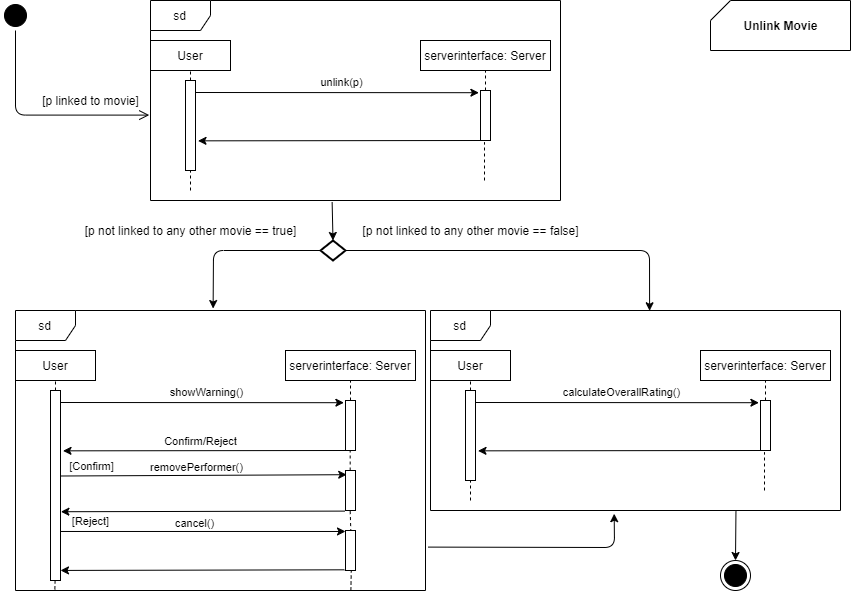
\includegraphics[width=\textwidth]{../images/topic3_iod.png}
	\caption{The interaction overview diagram}
	\label{iod}
\end{figure}

\begin{lstlisting}[caption={Contracts written in OCL},label={contracts2}]
	context Movie::unlink(performer)
	pre  self.performers[performer] -> not isEmpty()
	post self.performers[performer] -> isEmpty()
	
	context MovieManager::removePerformer(performer)
	pre forAll(movie | movie.performers[performer] -> isEmpty())
	post self.performers[performer] -> isEmpty()
	
	context Movie::calculateOverallRating()
	post self.overallRating = 0.5 * (self.mean(self.performers.getRatings()) + self.rating)
\end{lstlisting}

Based on the IOD and the specified contracts the CTS matrix gets defined and leads to the CTS shown in \autoref{cts}.

\begin{longtable}[h]{llll}
	Operations & Pre & Post & Composite States \\
	$O_{1}$ & $S_{0}$ & $S_{1}$ OR $S_{2}$ & A \\
	$O_{2}$ & $S_{1}$ & $S_{3}$ OR $S_{4}$ & B \\
	$O_{3}$ & $S_{3}$ OR $S_{4}$ & $S_{2}$ & \\
	$O_{3}$ & $S_{2}$ & $S_{5}$ & \\
\end{longtable}

The operations (sequence diagrams in the IOD) can be thought of as the transitions in the CTS, whereas the states match the specified postconditions (maybe thought of as starting points of arrows).

\begin{figure}[h]
	\centering
	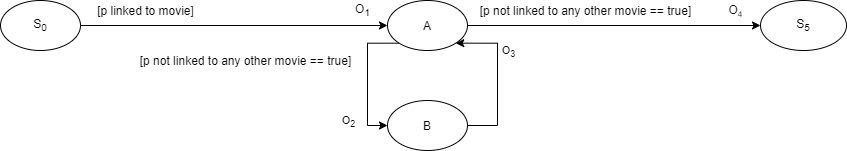
\includegraphics[width=\textwidth]{../images/topic3_cts.png}
	\caption{Contracts Transition System}
	\label{cts}
\end{figure}

For instance, the state $S_{0}$ describes the state when a performer p is linked to the given movie. One can then apply the operation $O_{1}$ to unlink the performer, resulting in the composite state A where either the performer is not linked to any other movie $S_{1}$ or the performer is still linked to another movie $S_{2}$.

Based on a coverage criterion the test paths get derived. Different from the first approach no test scenarios get generated. The paper only shows a new more low-level, graphical approach to generate test paths as this was even a suggested improvement from the authors of the first paper. 

\newpage
\section{Comparison} \label{comparison}
\begin{small}
\begin{longtable}[h]{p{0.45cm}|p{0.425\textwidth}|p{0.425\textwidth}}
	\caption{Synthesis matrix}
	\label{tab3:synthesismatrix}
	\\    %%%%<===
	\hline
	\textbf{No.} & \textbf{Approach 1} & \textbf{Approach 2} \\
	\hline
	1a) & 
	Use cases describing the basic operations in the transition system. Contracts that are attached to the use cases describing the states in the transition system. A contract consists of pre- and postconditions that specify the system properties to make a use case applicable and which properties are acquired by the system after its application. Parameters to contracts are actors and main concepts of the use case. The transition system (UCTS) itself as a simulation model to derive test objectives. The states in the UCTS are given through the predicates defined in the contracts, the transitions are triggered when applying an instantiated use case. Test objectives describing the test paths. Test objectives are derived by traversing the UCTS using a specific coverage criteria. Use case scenarios to build test scenarios from test objectives. Use case scenarios contain the main messages exchanged between the tester and the SUT, they define how the system has to be simulated to perform a use case and how to react to the simulation. & 
	IODs holding all scenarios and operations of a use case. Operations can either be interaction uses or sequence diagrams inside the IOD and define the state transitions. Contracts written in OCL that are attached to the operations describing the states in the transition system. The CTS describing the transition system. Test paths derived from the CTS using coverage criteria.  \\
	\hline
	1b) & 
	Use cases, contracts written as logical expressions, use case scenarios (sequence diagrams), initial system state, selected coverage criterion, and additional use case scenario parameters. & 
	IODs, contracts written in OCL, selected coverage criterion, possibly manual resolving of conflicts in the CTS matrix. \\
	\hline
	1c) &
	To express the ordering constraints between use cases, each use case is attached by a contract. To simulate the use cases, the set of formal parameters of the contracts are replaced with all possible combinations of their actual values. The use cases are then called \textit{instantiated}. To apply an instantiated use case the precondition of its contract must match with the current simulation state. Afterwards the simulation state is updated according to the postcondition of the use case. Exhaustively simulating the system results in the UCTS. To derive test objectives the transition system is traversed according to one of the predefined coverage criteria AE, AV, AIUC, AV-AIUC, or APT. To build test scenarios a use case scenario can replace a use case at a certain stage of execution if the state reached at this stage locally implies the precondition of the use case scenario. Executable test scenarios are generated by the prototype-tool UC-SCSystem. &
	Each operation in the IOD was enriched with its own contract written in OCL. To build the CTS, first all operations have to be identified from the IOD. The operations are taken from the sequence diagrams or from other operations expressed as interaction occurrences in the IOD. Using the contracts of operations, the states for the CTS are identified. Eventually, conflicts in the CTS have to be resolved such as logical if-then-else conditions, equal contract statements, or join nodes. After the CTS was built, test paths are derived from the CTS by applying a coverage criterion, which is either state-, transition- or transition pair coverage. \\
	\hline
	2a) & 
	Automatic test generation from use cases and use case scenarios. Requirement validation by identifying inconsistencies, underspecifications, and invariants. & 
	Deriving test paths from IODs. Further requirement validation on use case level.\\
	\hline
	2b) & 
	Test writers / Developers, Requirement Engineers. &
	Test writers / Developers, Requirement Engineers. \\
	\hline
	2c) &
	Software Requirements (definition of a software requirement, functional requirements, acceptance tests), Software Testing (model-based techniques, objectives of testing, evaluation of the tests performed), Software Engineering Models and Methods (preconditions, postconditions and invariants, behavioral modeling, analysis for consistency, and correctness, traceability). &
	Software Requirements (definition of a software requirement, functional requirements, acceptance tests), Software Testing (model-based techniques), Software Engineering Models and Methods (preconditions, postconditions and invariants, behavioral modeling, analysis for consistency and correctness). \\
	\hline
	3a) & 
	Dedicated editor to design use cases with contracts, UC-System to build the UCTS simulation model, and to derive test objectives from it. UC-SCSystem to exchange the use cases by use case scenarios in order to build the executable test case scenarios. & 
	UML 2.0 as a standard for IODs, OCL as a formal language to write the contracts, prototype tool to derive test paths. \\
	\hline
	3b) & 
	Writing the use cases and contracts is supported by a dedicated editor, but has to be done manually. Deriving test objectives from use cases and contracts through the transition system is done automatically by UC-System. Use case scenarios have to be specified manually, the generation of test scenarios works semi-automatically with UC-SCSystem as it may need additional parameters from the tester. & 
	Only the IOD and contract specification has to be done manually, the complete approach was then automized by a prototype tool. \\
	\hline
	4a) & 
	The approach was evaluated by looking at the statement coverage of three sample programs and the efficiency of test case scenario generation. & 
	The approach was evaluated by looking at the number of test paths generated to cover all success scenarios and fault detections. \\
	\hline
	4b) &
	Code coverage with the most coverage criteria was around 80\%. The coverage criteria differ in efficiency. AE, AV, and AV-AIUC perform with low efficiency, the sets of test cases are larger than in AIUC and APT. APT reaches 100\% functional test coverage with only 15 test case scenarios. Testing robustness leads to a high number of generated test case scenarios that only cover about 50\% of the corresponding code. The approach is good for functional testing, but bad for robustness testing. &
	Using the transition criterion to derive test paths leads to a reasonable amount of test paths and covers all alternative flows in the IOD, but is not suitable for fault detection at any time. The transition pair coverage criterion guarantees the maximum fault detection, but leads to a high amount of test paths. State coverage captures all success scenarios. \\
	\hline
\end{longtable}
\end{small}

Both approaches have a transition system as a core component in common. Both use contracts to define the states in the transition system. A transition can be applied in case the precondition is fulfilled, the state is then updated according to the postcondition. The transition system is used to derive test paths. Furthermore, both approaches define coverage criteria to generate a certain amount of test cases from the transition system. Both have the AE/transition coverage criterion and AV/state coverage criterion in common. Using this core idea it is also easy in both approaches for requirement engineers to validate their specified requirements during the simulation of the transition system. Both papers draw a similar conclusion, that the core approach is helpful to generate functional test case scenarios for the requirements, nevertheless, there is a lack to achieve a comparable coverage for robustness code for fault detection.

Nevertheless, the two approaches differ in their case of application. While \cite{ClementineNebut2006} uses use cases to automatically generate system-level tests, \cite{NajlaRaza2007} restricts to generate test paths for a specific use case. It therefore does not need additional use case scenarios as an input like \cite{ClementineNebut2006} to generate test scenarios as these are already natively given in the IOD. 

Besides the case of application, the input parameters in both approaches are different as well. \cite{ClementineNebut2006} uses requirement-level first-order logical expressions to describe use cases and their contracts. A more graphical approach was chosen in \cite{NajlaRaza2007} by specifying a use case with an IOD instead of using a formal language. 

\cite{ClementineNebut2006} has the special characteristic that it demonstrates an almost fully automized end-to-end test scenario generation process until concrete test execution, which is missing in \cite{NajlaRaza2007}. Nevertheless, this could easily be implemented in \cite{NajlaRaza2007} as well using similar tool support as in \cite{ClementineNebut2006}. 

\section{Conclusion} \label{conclusion}

Testing with a transition system delivers a method on how to bring requirement specification and system test generation closer together, eliminating traceability problems between what was specified and what was implemented. Requirements can easily be validated on their consistency, correctness, and on possible underspecification while at the same time test paths can be derived through traversing the transition system. 

\newpage

In literature search, a second paper besides the given one was found that follows the process of automatically generating test paths through traversing a transition system, but this time uses the in \cite{ClementineNebut2006} proposed extension of IODs as a form of activity diagrams instead of use cases as its input besides contracts. To find this article both snowballing and search-term-based techniques were used, whereas the choice of relevant articles was based on previously specified relevance criteria. Eight resulting papers were found according to these criteria, \cite{NajlaRaza2007} was finally chosen. 

Approach \cite{ClementineNebut2006} almost shows a fully automated way to derive executable test scenarios as JUnit tests. Contract enriched use cases using a formal language based on requirement-level first-order logical expressions are used as an input to the simulation model. Through exhaustive simulation, a transition system is build from which test objectives are derived using coverage criteria. It was empirically proven that the AIUC and APT criterion perform the most efficient and the most extensive measured by statement coverage. Giving contract enriched use case scenarios as a second input helps to generate concrete executable test scenarios. 

\cite{NajlaRaza2007} switches from system level to use case level test generation. It uses contract enriched IODs as graphical input and builds a transition system on it. Test paths are generated using the transition coverage criterion. No further methodology was introduced to generate executable test cases, but as the approach is already specified on use case level, the generation of test code is self-explanatory (a similar tool like UC-SCSystem from \cite{ClementineNebut2006} can be used).

One weakness of both approaches remains the capability to generate a sufficient amount of robustness tests for fault detection. Both approaches only rely on contract violations and do not sufficiently cover data variations as test path generation is only based on one initial state chosen by the test creator. Still, for the automatic generation of functional test scenarios, both approaches show industry-standard and highly applicable solutions.
